\section{LPWAN}
Per riuscire a gestire in maniera adeguata il sempre maggior numero di device
connessi, e le diverse problematiche che essi comportano, è necessario andare a
cambiare le topologie di rete per fare in modo che rispecchino i punti necessari
per garantire il corretto funzionamento. Finora le principali tecnologie
utilizzate erano la rete cellulare 2G, 3G, 4G, la quali hanno un ampia copertura
su tutto il territorio, ma devices che alimentati tramite batteria hanno durate
massime di mesi. Oltre alla rete cellulare abbiamo gli standard IEE 802.11, il
comunemente chiamato wifi, il quale garantisce una copertura di poche decine di
metri e favorisce una connessione veloce a discapito della durata della
batteria. Oppure, Bluetooth e ZigBee i quali hanno offrono una connessione
wireless con copertura di poche decine di metri. Oltre al fatto di una scarsa
copertura e di un elevato consumo di energia per comunicazione, tutte queste
tipologie di rete non sono scalabili cioè non sono ideate per supportare un
carico di milioni di devices connessi contemporaneamente. Per colmare il gap tra
tecnologie esistenti e le necessita di connettere milioni di devices diversi
standard sono stati proposti, per risolvere queste problematiche. Pur essendo
diversi, alla base di ognuno di essi vine attuata il concetto di del LPWAN
\emph{Low power area network}. LPWAN è un termine usato per identificare tutte
quelle reti che permettono di connettere un numero elevato di device in modo
wireless per chilometri di distanza, riuscendo comunque a mantenere basso il
consumo energetico richiesto per la comunicazione. Inoltre l'hardware utilizzato
in questo tipo di rete ha un consto di produzione relativamente basso ,
rendendole ottime per il mondo del IoT. Per raggiungere questi punti, è
necessario accettare dei compromessi sul numero di dati trasmissibili e sulla
banda utilizzata. 

\begin{figure}[h]
        \centering 
                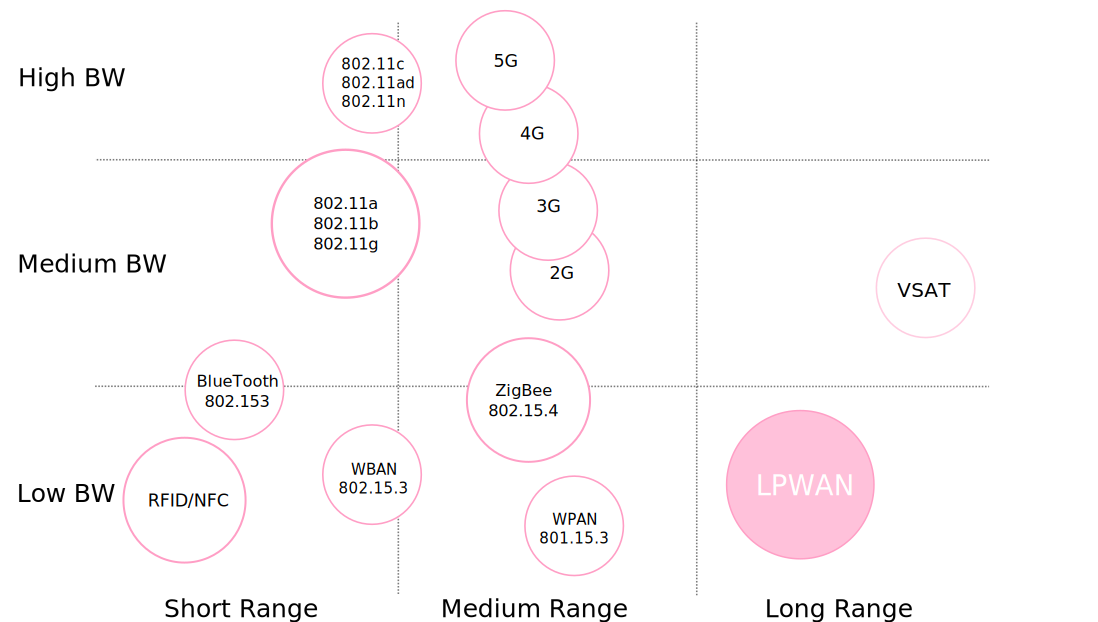
\includegraphics[width=16cm]{network_comp}
        \caption{Comparazione tipologia di reti}
\end{figure}

In questo contesto, i maggiori competitor sono Lora, Sigfox, NB-IoT e LTE-M.
Anche se ognuna di queste soluzioni punta a ottenere la più ampia fetta di
mercato, esse implementano soluzioni tecniche molto diverse tra di loro.
\subsection{NB-IoT e LTE-M}
NB-IoT e LTE-M, sono due nuovi standard certificati da 3GPP, entrambe questi
standard si basano su una versione modificata della rete 4G già esistente.
Quindi funzionano in uno spettro proprietario, e forniscono prestazioni diverse
per i diversi use-case. In particolare devices che utilizzano NB-IoT hanno una
durata della batteria molto più prolungata di quelli che utilizzano la
connessione LTE-M, la quale permette un maggiore band-with a discapito delle
durata. Il vantaggio di questi standard e che non servono grandi cambiamenti
alla rete telefonica, quindi sono facilmente implementabili dalle compagnie
telefoniche. Inoltre, ogni devices sarà dotato di una sim-card per poter
connettersi, in questo modo è possibile ottenere  una sicurezza simile a quella
implementato nelle connessioni LTE.
Altro punto a favore è il fatto che non è necessario utilizzare gateway, ogni
devices e connesso direttamente alla rete. 
La maggior parte delle compagnie telefoniche ha già dei piani per rendere disponibile queste due
tecnologie.

\begin{figure}[h]
        \centering 
                \includegraphics[width=11cm]{Comparsion_no_line}
        \caption{Comparazione tipologia di reti}
\end{figure}
\subsection{Sigfox}
Sigfox, azienda francese la quale offre una soluzione proprietaria per il mondo
del IoT. Sigfox opera sulle frequenze ISM, e punta a creare una rete a copertura
mondiale. Quello che promette questa tecnologia è un basso consumo energetico
per la comunicazioni andando a limitare di molto la banda utilizzabile per
l'invio dei dati. Sigfox utilizza una connessione \emph{Ultra narrow Band} ,
tramite la quale permette l'invio di un numero massimo di 140 messaggi per
giorno, con una lunghezza pari a 12 byte. Creando una rete globale problemi
quali compatibilità e roaming vengono superati andando ad offrire un piano unico
mondiale. Essendo il protocollo aperto, i vari moduli possono essere prodotti da
diverse compagnie andando a creare una concorrenza sul mercato e offrendo
diversi tipi di implementazione. I vari moduli sono disegnati per funzionare con
tecnologie già esistenti, andando a ridurre in maniera drastica il costo
unitario. Inoltre per come è strutturata la rete, i vari device possono
comunicare con le varie base station senza avere procedure di handshaking
rendendo effettivi i 140 messaggi giornalieri. La comunicazione tra device layer
e application layer è garantita da Sigfox stessa, lasciando al utente finale il
solo fatto di scrivere una semplice applicazione. Quindi la duplicazione dei
messaggi ricevuti e avviene in modo automatico , quando si ha un piano Sigfox.
Il range di azione varia da un paio di chilometri in zone urbane fino a decine 
di chilometri in zone rurali, dipende molto dalla topografia del terreno.
Supporta sia il l'uplink che il downlink ma entrambe le comunicazioni devono
essere inizializzate dal device. I messaggi non sono a lunghezza prestabilita,
quindi ogni messaggi varia in base al payload, payload più corti tempi di
comunicazione brevi. Il costo è basso perché l'approccio è open hardware, quindi
tutte le case produttrici di chip possono integrare la comunicazione Sigfox.
Ogni messaggio è firmato tramite una chiave unica proprietaria del device e il
fatto che non ci sono handshake nella comunicazione garantisce che le chiavi di
sicurezza non vengano intercettate da attacchi esterni. Ogni messaggio viene
inviato 3 volte per garantire la sicura ricezione. 
